\documentclass[a4wide]{report}

\usepackage{amsmath}
\usepackage[a4paper, total={7in, 10.2in}]{geometry}
\usepackage{graphicx}
\usepackage[portuguese]{babel}
\usepackage[utf8]{inputenc}


\begin{document}

\noindent
{\bf Rafael V. Cacilhas  - Relatório 01 (\today)}

\vspace{0.5cm}

\section*{Exercício 1}

O software produzido converte um número binário em linguagem de computador para um numero decimal e converte um numero decimal para a notação padrão de binário (não em linguagem de computador).

\subsection*{1 a) }
O numero binário que será convertido pode ser modificado editando o arquivo number.dat, bastando escrever cada dígito do número em uma linha diferente.

Foi feito um algoritmo para que o número em binário fosse lido diretamente de uma variavel integer, mas devido à grande extensão do algarismo (32 bits) não foi possivel criar uma variavel inteira tão grande e portanto o algoritmo não funciona para binários tão grandes.Ele foi deixado em comentário para quem se interesse.

Cada algarismo do numero é lido para uma posição de um array de tamanho 32 ( bin) e é em seguida separado em três partes: sinal ( bin(1)), expoente (bin(2) até bin(9)) e mantissa (bin(10) até bin(32)). Note que os arrays expo e mantiss invertem a ordem do array bin, por questão de conveniencia.

A saída do programa na tela é a conversão do número binário em decimal.

\subsection*{1 b) }

A conversão de decimal para binário é feita primeiramente separando o número decimal em sua parte puramente inteira e em sua parte puramente decimal. A parte inteira é trivial, pois o algoritmo de transformação em binário é extremamente simples.

A parte decimal traz o problema de não ser possível determinar de maneira simples quando o programa deve parar de rodar, pois o algoritmo não possui um fim explicito. A detecção de uma dízima não é simples de maneira geral, pois consiste em conferir todos os N-1 termos anteriores, o que é extremamente ineficiente para N grande. Foi escolhido utilizar um numero fixos de casas decimais (variavel precisao) e analisar caso a caso em busca de dízimas.
O número, convertido para binário, é escrito no arquivo bin.dat da mesma maneira que o arquivo fonte da letra a). Neste caso é 10011001011,1101110000.

 O número pedido não possui uma dízima, como foi verificado até a vigésima casa decimal. Apesar de ter sido calculado até a vigésima casa foi considerado desnecessário mostrar à partir da décima, devido ao grande número de zeros presentes; o erro associado é muito pequeno.



\section*{Exercício 2}
Com o objetivo de calcular o erro associado ao truncamento de uma variável foi definido o valor "exato" da subtração como sendo aquele feito com variaveis reais tipo *8. 

Para truncar na quinta casa decimal foi utilizado um pequeno truque: o valor da subtração foi multiplicado por $10^{3}$ de modo que o resultado tenha 5 casas decimais antes da vírgula. Em seguida esse valor foi salvo em uma variavel do tipo integer, de modo que as casas decimais fossem ignoradas. A seguir o valor foi transferido da variavel integer para uma variavel real*8 e dividido por $10^{3}$ de modo a ter somente as 5 casas decimais.

As saídas de dados na tela apresentam o resultado da subtração exato, truncado, erro absoluto e relativo entre eles. Como esperado a diferença entre a subtração exata e truncada se encontra na quinta casa decimal. Os valores de erro estão um pouco abaixo desta ordem de grandeza.

Naturalmente para uma conta simples desta não faz sentido o truncamento; mas é interessante ter o valor do erro para cálculos mais complexos. 


\section*{Exercício 3}
O software calcula o valor do somatório dado para variaveis real*4 e real*8. Vemos que na sétima casa decimal já há divergência entre os resultados.

Em seguida é calculado o mesmo somatório, mas começando dos maiores termos. A divergência entre real*4 e real*8 ocorre aproximadamente no mesmo local, na oitava casa. No entanto é possível perceber uma diferença enorme entre o resultado obtido neste cálculo e no cálculo anterior, sendo que o cálculo atual possui quase 100$\%$ de erro relativo ao valor calculado anteriormente.


\section*{Exercício 4}

Temos abaixo a equação de Van der Waals.
\begin{equation}
\left( p + \frac{N^{2}a'}{V^{2}}		\right)			\left( V - Nb'		\right) = Nk_{b}T
~~~~~~~.
\label{pressao1}
\end{equation}

\subsection*{a)}
Segue os gráficos para T = Tc/2, T = Tc e T = 3*Tc/2 para dois ranges de volume diferentes.


\begin{figure}[h]
\centering
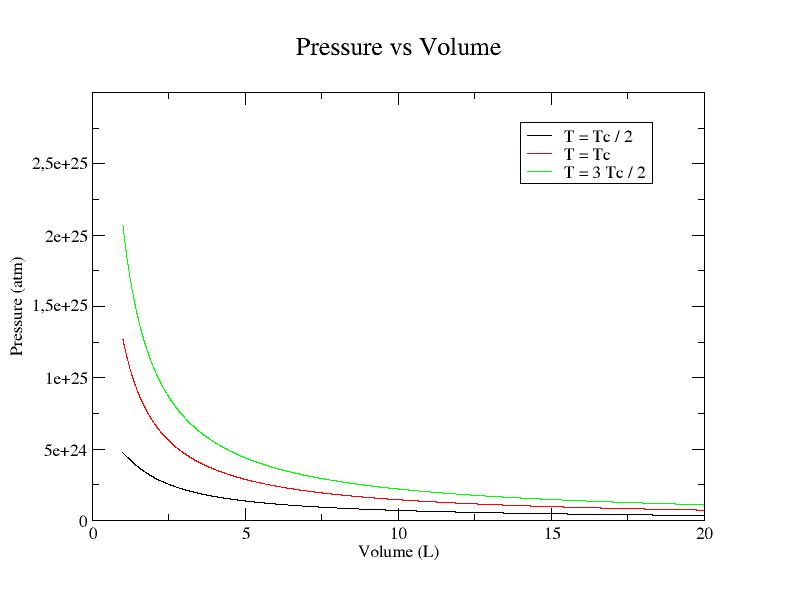
\includegraphics[width=0.45\textwidth]{v_alto.jpg}%
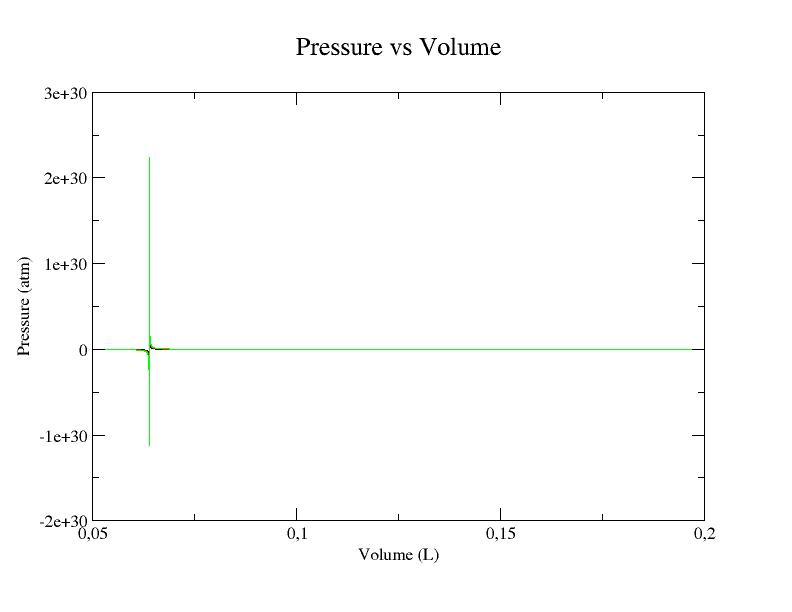
\includegraphics[width=0.447\textwidth]{v_baixo.jpg}
\caption{Pressão em função do volume para dois ranges de volume.}
\label{p1}
\end{figure}

\subsection*{b)}

Definindo $T' = \frac{T}{T_{c}}$,$p' = \frac{p}{p_{c}}$ e $V' = \frac{V}{V_{c}}$, onde $T_{c} =\frac{27k_{b}b'}{8a'}$, $p_{c} =\frac{a'}{27b'^{2}}$ e $V_{c} =3Nb'$ e multiplicando os dois lados da equação por $\frac{27k_{b}b'}{8a'}$, podemos reescrever a equação como:


\begin{equation}
\left( p' + \frac{3}{8V'^{2}}		\right)			\left( V' - \frac{1}{3}		\right) =3T'
~~~~~~~.
\label{pressao2}
\end{equation}
Abaixo seguem os graficos de P' em função de V'.

\begin{figure}[h]
\centering
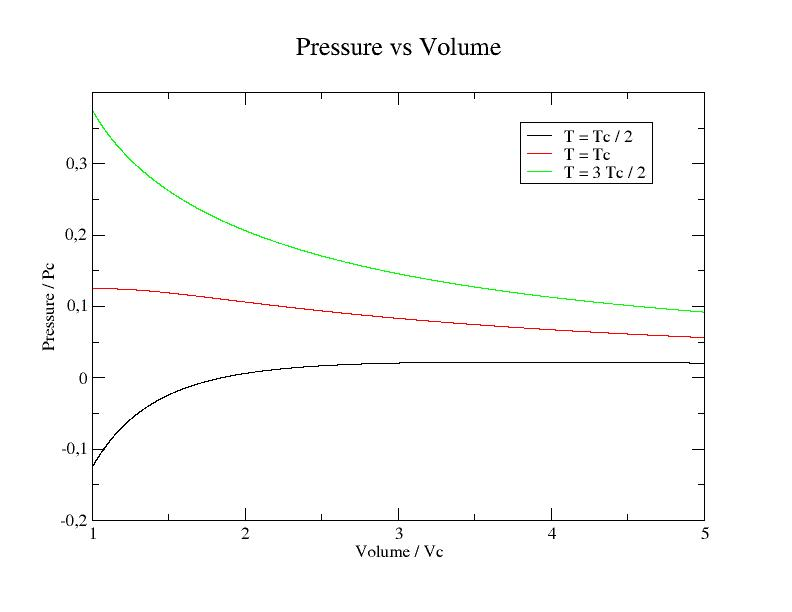
\includegraphics[width=0.45\textwidth]{v_alto2.jpg}%
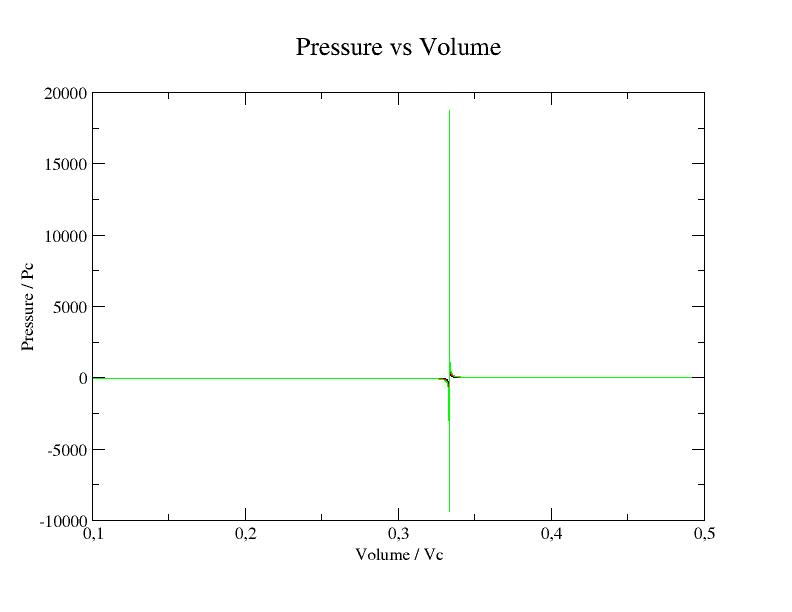
\includegraphics[width=0.447\textwidth]{v_baixo2.jpg}
\caption{Pressão em função do volume para dois ranges de volume.}
\label{p2}
\end{figure}


	Como podemos ver na Figura \ref{p2} o uso das variaveis auxiliares faz com que as grandezas P' e V' tenham aproximadamente a mesma ordem de grandeza, fato que auxilia na compreensão do gráfico, além de fazer com que P não tenha valores extremamente altos, o que ajuda no cálculo computacional. Além disso, escrever a pressão como P' = P / Pc faz com que o comportamento das curvas em temperaturas diferentes seja drásticamente diferente, onde vemos que para T = Tc/2, abaixo de V' = 2, temos a separação das três curvas, o que não ocorre no caso da Figura \ref{p1}. Por fim, a separação também traz facilidade no entendimento da expressão analítica, onde agora fica claro que a função deve divergir perto de V' = 1/3, fato que não é tão explícito (ao menos não em termos do valor numérico) na equação \ref{pressao1}.
	


\section*{Exercicio 5}
Não consegui aplicar a soma ao problema proposto, pois o algoritmo da soma trabalha com a soma de dois números, dados em log. O cálculo da função de partição trabalha com Z, não com logZ. Se tentarmos aplicar o log, ficamos com:

\begin{equation}
Z = Z_{1} + Z_{2} + Z_{3} + ... + Z_{n}
~~~~~~~.
\label{z}
\end{equation}

\begin{equation}
logZ = log (Z_{1} + Z_{2} + Z_{3} + ... + Z_{n} )
~~~~~~~.
\label{z2}
\end{equation}

Como o log da soma não é a soma dos logs não vejo como aplicar o algoritmo da soma para este caso, visto que o lado direito não é a soma de dois logs.
	
\section*{Exercicio 6}
\subsection*{a)}

\begin{equation}
S = \sum_{k=1}^{N}  [a*x_{k} + b - y_{k}]^2
~~~~~~~.
\label{regressao}
\end{equation}
	
Derivando em relação a a e b, temos:

	\begin{equation}
\frac{\partial S}{\partial a} = 2\sum_{k=1}^{N}  [ax_{k} + b - y_{k}]x_{k}
~~~~~~~.
\label{dsda}
\end{equation}
	\begin{equation}
\frac{\partial S}{\partial b} = 2\sum_{k=1}^{N}  [ax_{k} + b - y_{k}]
~~~~~~~.
\label{dsdb}
\end{equation}	


	
Separando os três termos do somatório e igualando a zero (pois queremos o mínimo), temos:	

	\begin{equation}
0 = \sum_{k=1}^{N} ax_{k}^{2} +\sum_{k=1}^{N} bx_{k} -\sum_{k=1}^{N}  y_{k}x_{k}
~~~~~~~.
\label{dsda0}
\end{equation}	

\begin{equation}
0 = \sum_{k=1}^{N} ax_{k} +\sum_{k=1}^{N} b -\sum_{k=1}^{N}  y_{k}
\label{dsdb0}
\end{equation}	
	
Vamos definir A = $\sumx$, A = $\sum x$, B = $\sum y$, C = $\sum x^{2}$ e D = $\sum xy$. Assim, o sistema fica da forma:

\begin{equation}
aC + bA - D = 0
\end{equation}

\begin{equation}
aA + Nb - B = 0
\end{equation}

Cujas soluções são:

\begin{equation}
a = \frac{ND - AB}{NC -A^{2}}
\end{equation}

\begin{equation}
b = \frac{BC - AD}{NC - A^{2}}
\end{equation}

Note que se quisermos forçar b = 0, temos que $B = \frac{AD}{C}$ e temos que:

\begin{equation}
a_{b=0} = \frac{ND - \frac{A^{2}D}{C}}{NC -A^{2}}
\end{equation}

\subsection*{b}
A saída do programa apresenta primeiramente na tela os valores do coeficiente angular a e o coeficiente linear b.
A equação da reta obtida pelo Grace é	 y = 1.6382 * x + 0.029209, onde vemos que o coeficiente angular bateu até a ultima casa de precisão do Grace, mas o coeficiente linear apresentou diferença já na segunda casa decimal.


\subsection*{c)}
A segunda linha da saída do programa é o coeficiente angular quando forçamos b = 0. Como o b encontrado foi maior que zero, temos que a possui um valor ligeiramente maior do que o encontrado anteriormente, como esperado.

O cálculo analítico já foi apresentado na letra a).

\subsection*{d)}
O coeficiente angular do experimento de Millikan representa a razão entre a massa das gotículas e a carga do elétron. Como não temos a unidade da massa utilizada o valor absoluto da razão não faz sentido, sendo que podemos então ignorar o expoente e trabalhar com o valor numérico. Comparando o valor numérico (esquecendo os expoentes) do coeficiente angular com a carga do elétron, temos que o experimento apresenta um erro relativo da ordem de 2$\%$



\section*{Exercicio 7}
\subsection*{a)}
A equação da reta encontrada pelo Grace é y = 67.415 * x + 758.39.
A saída do programa mostra primeiramente os resultados do fit através da rotina do Exercicio 6. Como podemos ver, a = 66.772 e b = 908.71. Os resultados de a discordam do Grace na segunda casa decimal e os de b discordam até mesmo na primeira.

\subsection*{b)}
O software foi feito seguindo a dedução analítica do Recipe e reescrevendo o algoritmo para FORTRAN90. Os resultados do calculo do coeficiente angular parecem coerentes, mas o erro calculado é bem grande, o que torna dificil saber se o algoritmo foi feito com sucesso.  O cálculo e erro do coeficiente linear b estão bem fora dos valores esperados pelo fit do Grace.

Infelizmente não consigo encontrar nenhum erro no algoritmo.



















\end{document}
